\likechapter{Введение}

Работа над выпускным квалификационным проектом происходила в Национальном Исследовательском Ядерном Университете «МИФИ» 
на кафедре № 5.

Целью выпускной квалификационной работы является разработка модели \ac{ascro} для полномасштабных тренажеров действующих 
\ac{aes}.

В связи с поставленной целью в ходе работы решаются следующие задачи:

\begin{itemize}
	\item изучение литературы, посвященной активации теплоносителя первого контура;
	\item разработка модели образования радиоактивных нуклидов в топливе ядерного реактора с дальнейшим переходом в
		теплоноситель первого контура;
	\item разработка модуля анализа свойств местности, прилегающей к \ac{aes}, по данным топологических карт;
	\item разработка расчетной сетки, описывающей прилегающую к \ac{aes} местность;
	\item аппроксимация свойств местности на узлы расчетной сетки;
	\item разработка модуля расчета мощности эквивалентной дозы внешнего гамма - излучения.
\end{itemize}

Ряд событий в прошлом, связанных с авариями на предприятиях атомной энергетики, показали необходимость создания систем 
\ac{ascro}. В современном мире системы \ac{ascro} являются неотъемлемой частью действующих \ac{aes}. 

С целью профессиональной подготовки и поддержания квалификации персонала \ac{aes}, возникла задача разработки модели 
\ac{ascro} для полномасштабных тренажеров действующих \ac{aes}. Задача является актуальной и новой, так как на данный 
момент на полномасштабных тренажерах Нововоронежской, Калининской и Ростовской \ac{aes} отсутствует возможность 
моделирования выхода радиоактивных веществ за пределы гермообъема и их дальнейшего распространения в атмосфере. Ценность 
разработки заключается в повышении квалификации персонала, руководства \ac{aes} и поддержании, улучшении навыков 
реагирования в случае возникновения аварийной ситуации на \ac{aes} для минимизации последствий аварии для населения, 
проживающего в городах-спутниках действующих \ac{aes}.

\textbf{Обзор литературы.} Проведем обзор имеющейся литературы в соответствии с поставленными задачами.

При изучении радиоактивных нуклидов, которые образуются в ядерном реакторе, важно учитывать не только продукты реакции 
деления $(n, f)$, но и радионуклиды, образующиеся в результате реакций превращения типа $(n, \gamma)$, $(n, 2n)$ на 
радиоактивных и стабильных изотопах в ядерном реакторе. <<Каждый нуклид, находящийся в работающем ядерном реакторе, в 
общем случае испытывает, кроме радиоактивного распада, ряд превращений, обусловленных взаимодействием с нейтронами: 
деление $(n, f)$, радиационный захват $(n, \gamma)$, реакцию $(n, 2n)$ и т.д.>> \citep[с.~6]{kolobashkin}.  
Авторы \cite{kolobashkin} выделяют более 650 радиоактивных нуклидов, массовые числа которых лежат в интервале от 72 до 
166, и около 60 актиноидов, которые генерируются в процессе работы ядерного реактора.

Радионуклидный состав и радиационные характеристики продуктов реакций деления и превращения в большинстве своем зависят 
от типа ядерного реактора и его особенностей. В источнике \cite{gusev_bio} описываются радионуклиды, образующиеся в 
ядерных реакторах типа \ac{vver} (\acl{vver}) и \ac{rbmk} (\acl{rbmk}), а так же радиационные характеристики этих 
нуклидов. Основными радионуклидами, образующимися в топливе во время работы ядерного реактора и играющими существенную 
роль в создании радиационной обстановки вблизи \ac{aes}, являются изотопы иода (I), а также \ac{irg} (\acl{irg}), а 
именно криптон (Kr) и ксенон (Xe).

Согласно \cite{gusev_bio, gusev_def, egorov}, помимо образования радиоактивных нуклидов в \ac{tvel}ах (\acl{tvel}), 
в ядерном реакторе присутствуют радионуклиды активационного и коррозионного происхождения. Как правило, такие нуклиды 
накапливаются в системе теплоносителя. Активность этой системы обусловлена следующими факторами:

\begin{itemize}
	\item собственная активность системы теплоносителя образуется из-за активации нейтронами ядер теплоносителя и 
		входящих в него естественных примесей;
	\item активность продуктов коррозии металлов (процесс коррозии в ядерном реакторе происходит на поверхности 
		конструктивных материалов \ac{az} (\acl{az}) и в системе теплоносителя);
	\item активность продуктов деления и актиноидов, проникающих через поврежденную или негерметичную оболочку 
		\ac{tvel}ов.
\end{itemize}
Для реакторов, охлаждаемых легкой водой, основной вклад как по удельной активности, так и по мощности дозы $\gamma$ - 
излучения среди нуклидов активационного происхождения является радионуклид $^{16}\text{N}$, который образуется в
активной зоне в результате реакции $^{16}\text{O}$(n, p)$^{16}\text{N}$. Эта реакция является 
пороговой и проходит при энергии нейтронов выше 10 МэВ. Также не менее важным нуклидом активационного происхождения 
является нуклид $^{41}\text{Ar}$, образуемый в реакции $^{40}\text{Ar}$(n, $\gamma$)$^{41}\text{Ar}$.

При моделировании процесса переноса радиоактивных примесей в атмосфере необходимо учитывать множество факторов и 
метеорологических особенностей переноса веществ. <<Примесью в метеорологии обычно называют вещества, удаляемые в 
атмосферу в виде газов и  аэрозолей в процессе выброса>> \cite[с. 52]{gusev_bio}. После попадания в атмосферу такие 
вещества распространяются в результате ветрового переноса и турбулентной диффузии. 

Ветровой перенос примесей при их непрерывном истечении из источника создает своего рода струю выброса, в то время как 
при слабом или отсутствующем ветре вокруг источника выброса образуется облако примесей, обусловленное превалированием 
диффузии над ветровым переносом. Турбулентность диффузии в атмосфере обусловлена наличием в атмосфере беспорядочных 
завихрений различных размеров и форм, источником которых являются силы трения, возникающие при взаимодействии ветрового 
потока с землей, а так же потоки воздуха, распространяющиеся в вертикальном направлении вблизи нагретой поверхности. 
Взаимодействие атмосферных вихрей с облаком выброса зависит от отношения размеров вихрей и облака. \cite{gusev_bio}

При наличии ветра основной вклад в формировании турбулентности вносят силы трения ветровых потоков с поверхностью земли. 
Такой тип турбулентности называют \textit{механической}. Интенсивность данного типа турбулентности зависит от скорости 
ветра, но в большей степени от рельефа поверхности земли. Влияние рельефа поверхности на рассеяние примесей описывают 
величиной, называемой шероховатостью подстилающей поверхности или высотой подстилающей поверхности $z_0$. Согласно 
\cite{setton, bizova_meteor, berlyand}, высота подстилающей поверхности рассчитывается по вертикальному профилю ветра в 
приземном слое воздуха при нейтральных условиях, однако на практике при метеорологических расчетах используют табличные 
значения \cite{mlyavaya} (см. приложение А). Качественная картина поведения примеси при выбросе в атмосферу изображена 
на рисунке \ref{fig_emissions}.

\begin{figure}[ht]
\centering
	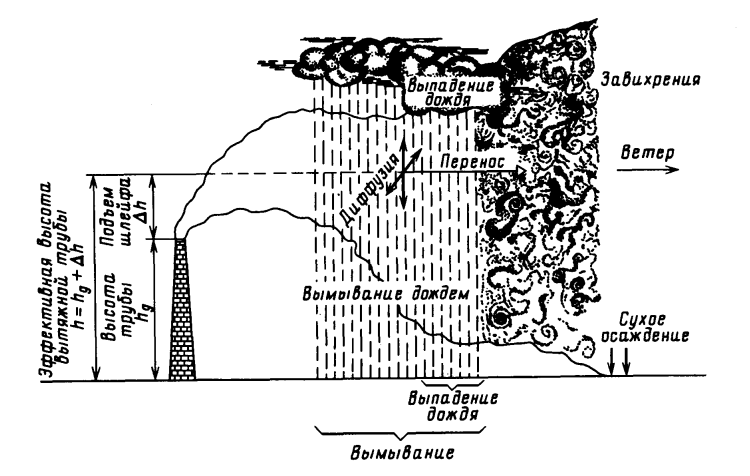
\includegraphics[width=13cm]{emissions}
	\captionsetup{justification=centering}
    \caption{Картина поведения примеси, выбрасываемой в атмосферу \cite{gusev_bio}.}
    \label{fig_emissions}
\end{figure}

Согласно \cite{gusev_bio}, математическое моделирование диффузии примесей в атмосферы рассматривается в двух вариантах: 
\begin{itemize}
	\item статистическое моделирование (Гаусова модель);
	\item решение дифференциальных уравнений переноса примесей.
\end{itemize}

Так как при рассмотрении турбулентной диффузии в атмосфере необходимо учитывать множество труднопредсказуемых факторов, 
учесть их все в рамках одной модели не представляется возможным. В связи с этим в современном мире существует множество 
различных моделей рассеяния примесей в атмосфере, каждая из которых обладает своими достоинствами и недостатками. 
Подробное описание существующих моделей рассеяния примесей изложены в источниках \cite{setton, bizova_meteor, berlyand, 
radio_transfer, disper_atmos, met_radio, general_exposure, laihtman, bizova_scatter, disper_models}.

Одной из главных задач современных систем \ac{ascro} на \ac{aes} является измерение значений мощности дозы 
гамма - излучения на прилегающей к \ac{aes} местности. Методика расчета мощности эквивалентной дозы внешнего гамма - 
излучения при разработке модели \ac{ascro} представлена в источнике \cite{elokhin}. 

Измерение мощности эквивалентной дозы внешнего гамма - излучения производится специализированными датчиками фотонного 
излучения, расположенными на прилегающей к \ac{aes} местности \cite{elokhin}. При проектировании системы используются 
блоки детектирования типа БДМГ-08Р3, БДМГ-08Р4, БДМГ-08Р5, БДМГ-100. Технические характеристики, принцип работы датчика 
фотонного излучения БДМГ-100 представлен в источнике \cite{bdmg-100}.

\textbf{Обзор программных средств}. Проведем обзор программных средств, которые используются в ходе работы над выпускным 
квалификационным проектом. 

В начале работы над выпускной квалификационной работой ставится задача разработки модели образования радиоактивных 
нуклидов в топливе ядерного реактора с дальнейшим переходом в теплоноситель первого контура, в результате которой будут 
получены концентрации радионуклидов в теплоносителе первого контура. Для расчета концентраций необходимо знать двухгрупповые 
микроскопические сечения реакций, приводящих к образованию радионуклидов. С целью расчета таких сечений используется 
программа UNK \cite{unk}, позволяющая получить усредненные двухгрупповые сечения реакций. Программа UNK предназначена 
для расчета нейтронно-физических характеристик ячеек и ТВС ядерных реакторов различного типа. Библиотека ядерных данных 
программы включает около 300 изотопов и рассчитана с помощью программы NJOY из файлов оцененных данных ENDF/B-VI, 
JEFF-2.2 и JENDL-3.2.

Предполагается, что модель \ac{ascro} будет основана на том, что распределение примесей в атмосфере описывается 
полуэмпирическим уравнением адвекции-диффузии \cite{elokhin}. Это уравнения является дифференциальным уравнением в 
частных производных. 

Существует ряд методов, которые позволяют численно решать дифференциальные уравнения в частных производных. В данной 
работе для решения поставленных задач был выбран метод конечных элементов \cite{mke}. В основе метода конечных 
элементов лежит принцип разделения исследуемой области на подобласти (рисунок \ref{fig_mesh}). Метод обладает рядом 
преимуществ для рассматриваемой задачи:

\begin{itemize}
	\item универсальность метода позволяет решать практически любые краевые задачи;
	\item метод позволяет решать дифференциальные уравнения для области любой сложности;
	\item в особенно важных подобластях есть возможность повысить плотность расчетной сетки для увеличения точности 
		вычислений, в то время как в менее важных областях понизить плотность сетки для снижения затрат процессорного 
		времени. 
\end{itemize}

\begin{figure}[ht]
\centering
	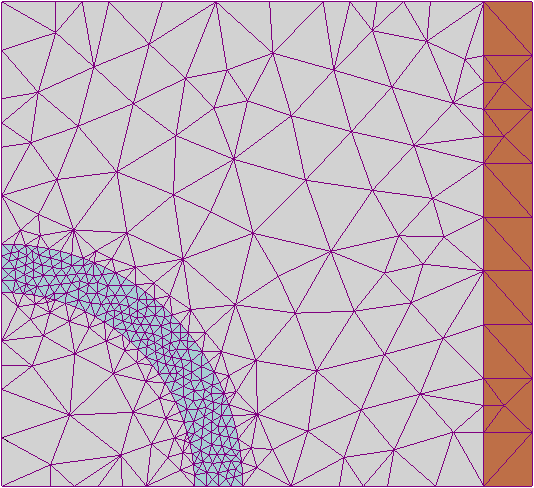
\includegraphics[width=8cm]{2D_mesh}
	\captionsetup{justification=centering}
    \caption{Разбиение области на конечные элементы \cite{wiki_mke_fig}.}
    \label{fig_mesh}
\end{figure}


Для численного моделирования физических процессов, которые можно описать при помощи дифференциальных уравнений в 
частных производных, существует множество пакетов и программных средств. Одним из них является вычислительный пакет 
FEniCS \cite{fenics_tut1}. Проект FEniCS разрабатывался группой исследователей из институтов со всего мира и имеет 
большой список возможностей, позволяющих автоматизировать решение дифференциальных уравнений. К достоинствам пакета 
FEniCS можно отнести:

\begin{itemize}
	\item содержание обширной документации, большое сообщество и простой синтаксис, что обеспечивает низкий порог 
		вхождения;
	\item возможность использования языков программирования Python и C++ для проведения расчетов;
	\item высокопроизводительная алгебра, параллельные вычисления, позволяющие снизить затраты процессорного времени; 
	\item автоматическое решение дифференциальных уравнений;
	\item возможность расчета на 1, 2 и 3-х мерных сетках;
	\item простота установки пакета.
\end{itemize}

В качестве языка программирования для решения дифференциального уравнения методом конечных элементов был выбран язык 
Python \cite{python_lutz}. Python - язык программирования высокого уровня. Синтаксис языка достаточно прост, что 
позволяет не отвлекаться от решаемой задачи на особенности языка и увеличивает скорость разработки. Python идеально 
подходит для программирования математических вычислений, так как обладает обширной библиотекой, предоставляющей массу 
возможностей, востребованных в вычислительных программах. Помимо стандартной библиотеки, Python допускает расширение 
возможностей как за счет своих собственных библиотек, так и за счет библиотек, созданных сторонними разработчиками. 
Одним из важнейших критериев выбора языка стала поддержка пакетом FEniCS языка программирования Python. К тому же, 
Python имеет возможность работать с такими языками, как Fortan и C++, которые активно используются в научных расчетах.

Создание расчетной сетки для решения дифференциального уравнения методом конечных элементов может стать непростой 
задачей, если требуется смоделировать 3-х мерную геометрию с повышением и понижением плотности сетки в различных 
областях. Для решения этой задачи существует программа gmsh \cite{gmsh_man}, которая и используется в данной работе.
Gmsh - программа, позволяющая генерировать расчетные сетки любой сложности. Основная цель gmsh - предоставить 
пользователю простой, быстрый и удобный инструмент для создания сетки с параметрическими входными данными.

Для того, чтобы задать параметры расчетной сетки, в gmsh присутствует модуль геометрии. При генерации расчетной сетки 
необходимо создать файл, содержащий команды на скриптовом языке gmsh, в котором детально описываются опорные точки и 
линии создаваемой геометрии. Для создания такого файла в текущей работе используется сторонняя библиотека для языка 
python, которая называется pygmsh \cite{pygmsh_doc}. Эта библиотека является мощным инструментом, предоставляющим 
интерфейс для скриптового языка gmsh. Помимо удобных абстракций, библиотека содержит множество примеров создания 
расчетных сеток различной сложности. Более того, из за гибкости языка программирования python, имеется возможность 
параметризировать создание расчетной сетки и в дальнейшем при необходимости менять её параметры без изменения скриптового 
файла gmsh.